\chapter{Level 4: Network defence}
At this level, we implemented network defence mechanisms to mitigate the impact of the TCP SYN Flood and ICMP Flood attacks demonstrated at the previous level. We utilised the Linux firewall tool \texttt{iptables} to configure firewall rules on the victim machines to protect against these attacks.

\section{Firewall Configuration}
\subsection{TCP SYN Flood Attack with IP Spoofing}
To defend against the TCP SYN Flood attack with IP spoofing, we implemented the following firewall rules using \texttt{iptables}:

\begin{verbatim}
sudo iptables -A INPUT -p tcp --syn -m limit 
--limit 1/s --limit-burst 4 -j ACCEPT
sudo iptables -A INPUT -p tcp --syn -j LOG 
--log-prefix 'TCP SYN FLOOD DROPPED:' --log-level 4
sudo iptables -A INPUT -p tcp --syn -j DROP
\end{verbatim}

These rules limit the rate of incoming TCP SYN packets to 1 packet per second, with a burst limit of 4 packets. Any TCP SYN packets exceeding this limit are logged with a specific prefix and dropped. This configuration helps prevent the victim machines from being overwhelmed by the flood of SYN packets the attacker generates.

\subsection{ICMP Flood Attack}
To mitigate the ICMP Flood attack, we applied the following \texttt{iptables} rules:

\begin{verbatim}
sudo iptables -A INPUT -p icmp --ICMP-type echo-request -m limit 
--limit 1/s --limit-burst 4 -j ACCEPT
sudo iptables -A INPUT -p icmp --ICMP-type echo-request -j LOG 
--log-prefix 'ICMP FLOOD DROPPED:' --log-level 4
sudo iptables -A INPUT -p icmp --ICMP-type echo-request -j DROP
\end{verbatim}

Similar to the TCP SYN Flood defence, these rules limit the rate of incoming ICMP echo request packets to 1 packet per second, with a burst limit of 4 packets. ICMP echo request packets exceeding this limit are logged and dropped, protecting the victim machines from being overwhelmed by the ICMP Flood attack.

\section{Dropped Packets}
To verify the effectiveness of the firewall rules, we can examine the dropped packets using the following commands:

\begin{verbatim}
dmesg | grep 'TCP SYN FLOOD DROPPED'
dmesg | grep 'ICMP FLOOD DROPPED'
\end{verbatim}

Figure~\ref{fig:TCPSYNFloodDroppedPackets} shows the output of the first command, indicating that the firewall successfully dropped a significant number of TCP SYN packets during the attack.

\begin{figure}[H]
\centering
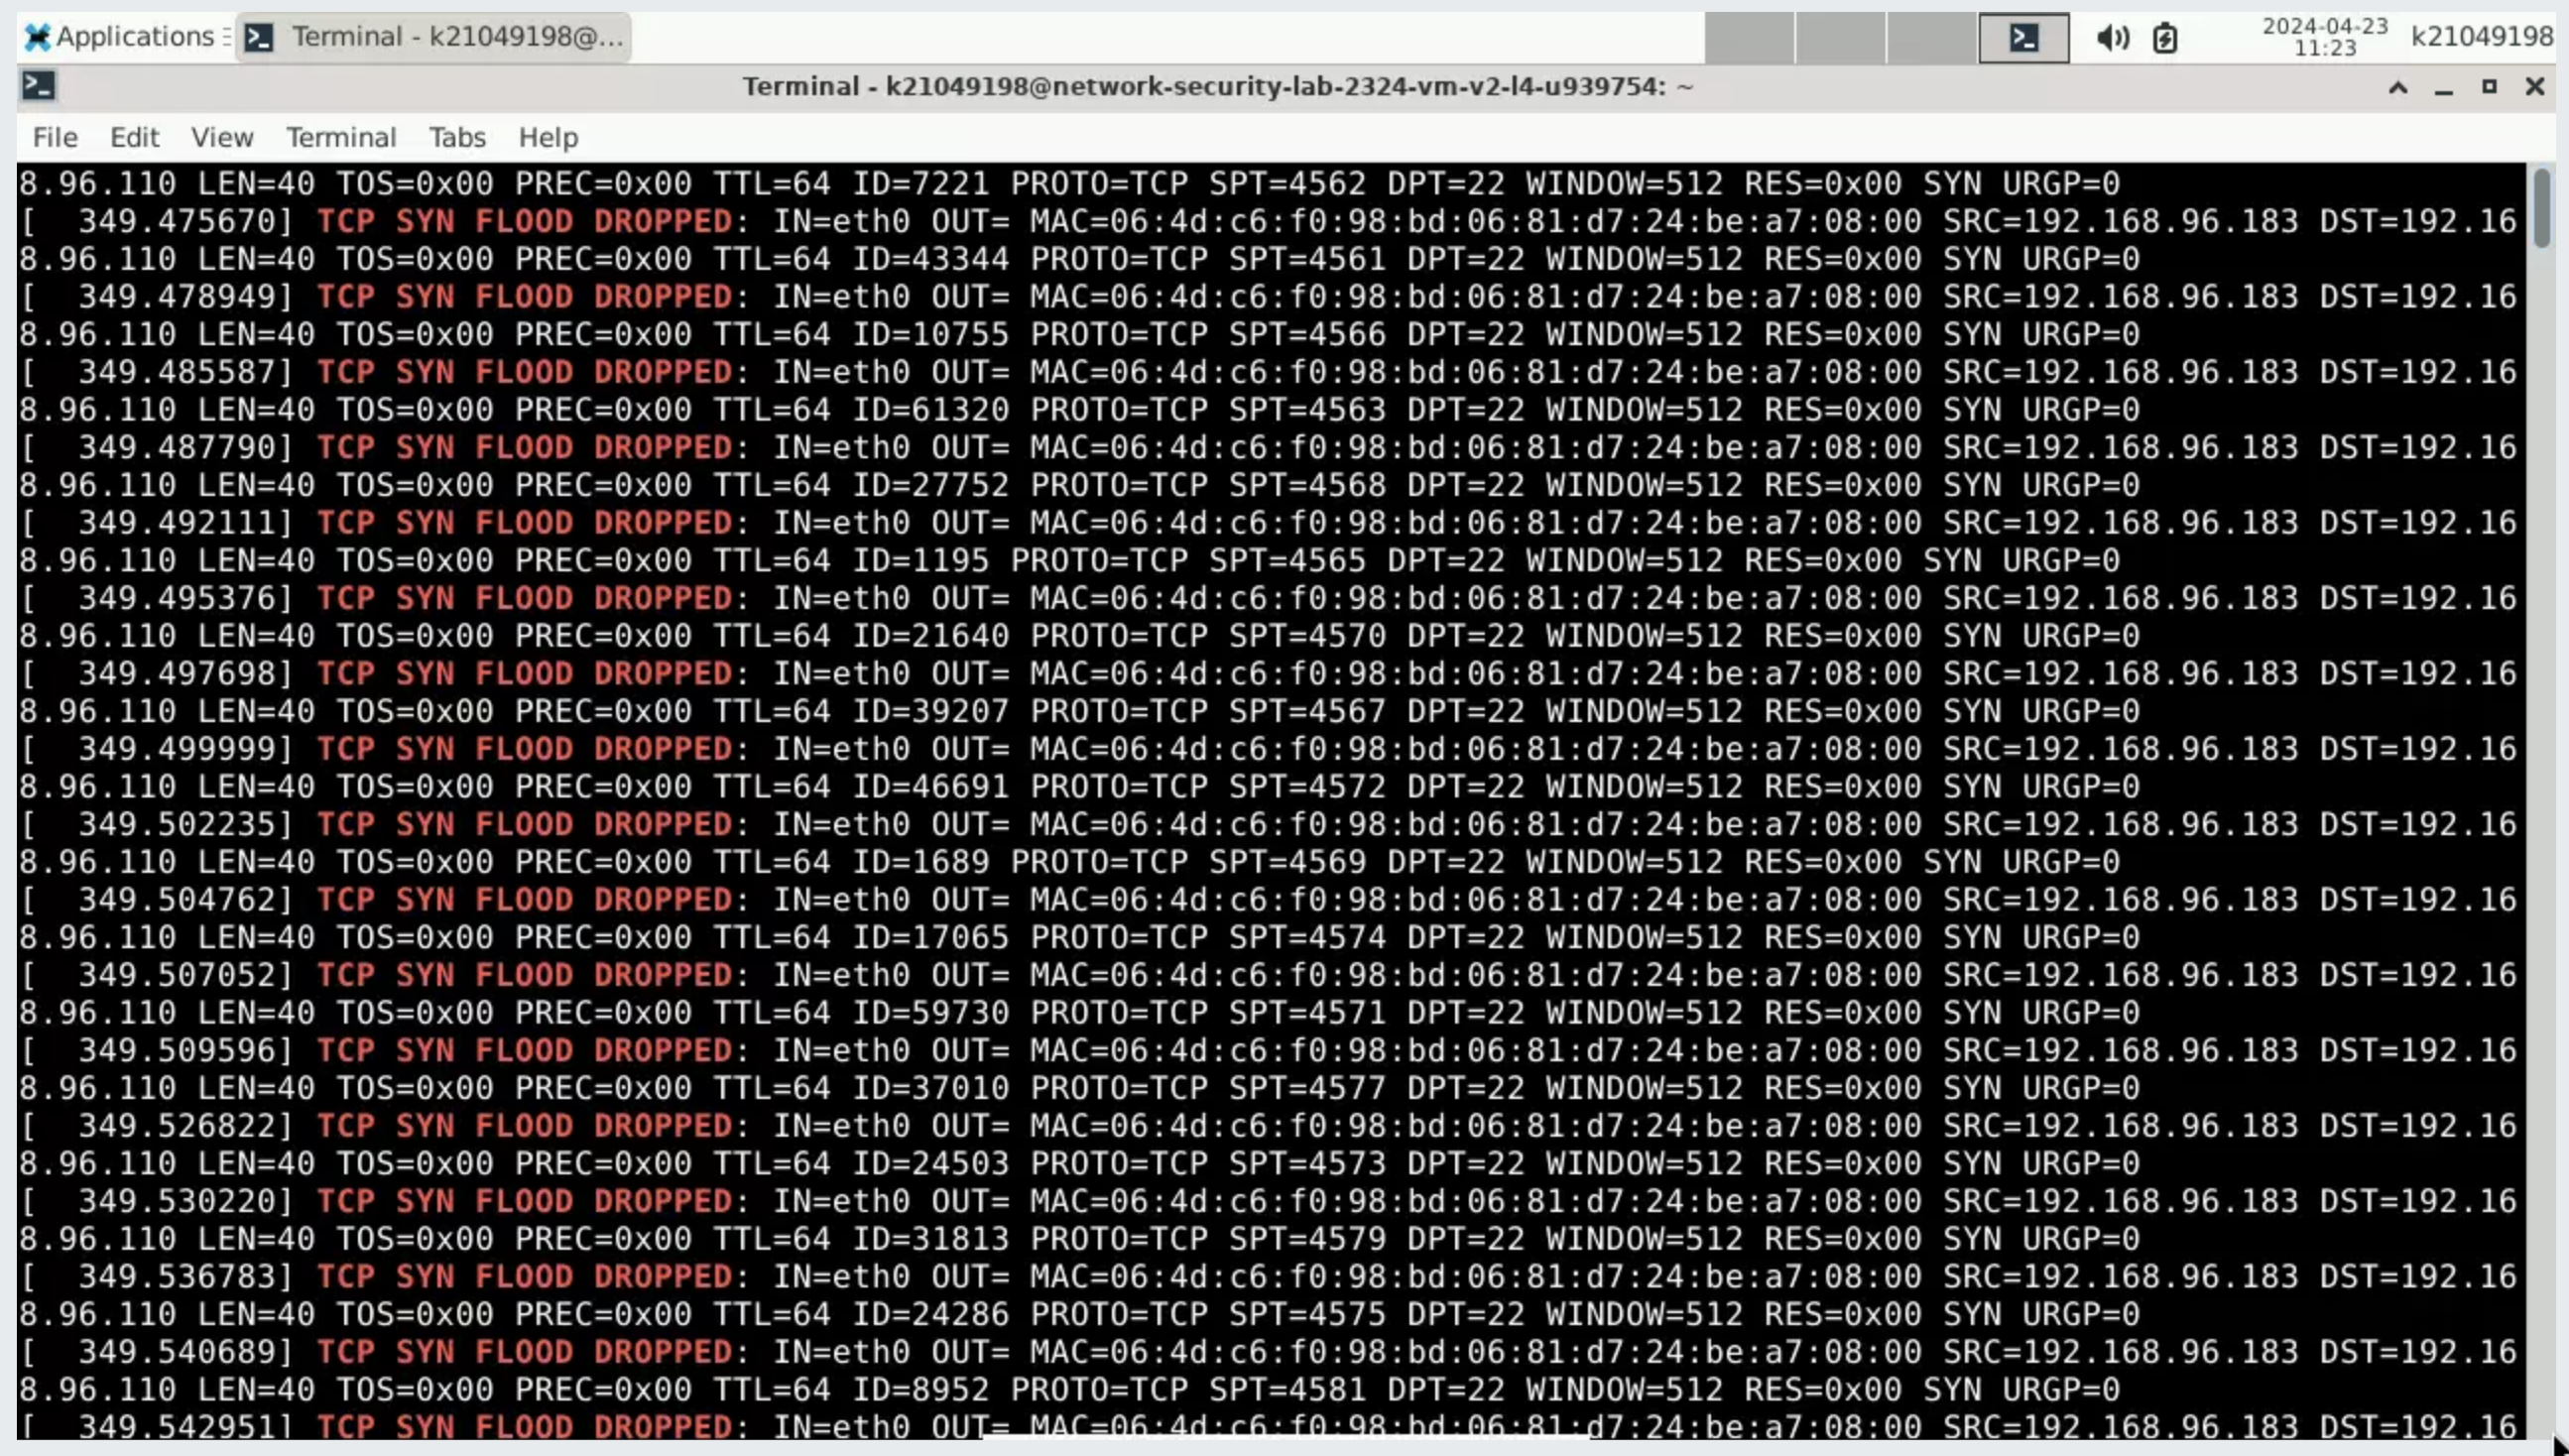
\includegraphics[width=0.8\textwidth]{img/level4/level4-dropped-packets-TCPSYNFlood.png}
\caption{Dropped Packets (TCP SYN Flood)}\label{fig:TCPSYNFloodDroppedPackets}
\end{figure}

Similarly, Figure~\ref{fig:ICMPFloodDroppedPackets} displays the output of the second command, confirming that the firewall effectively dropped many ICMP echo request packets during the ICMP Flood attack.

\begin{figure}[H]
\centering
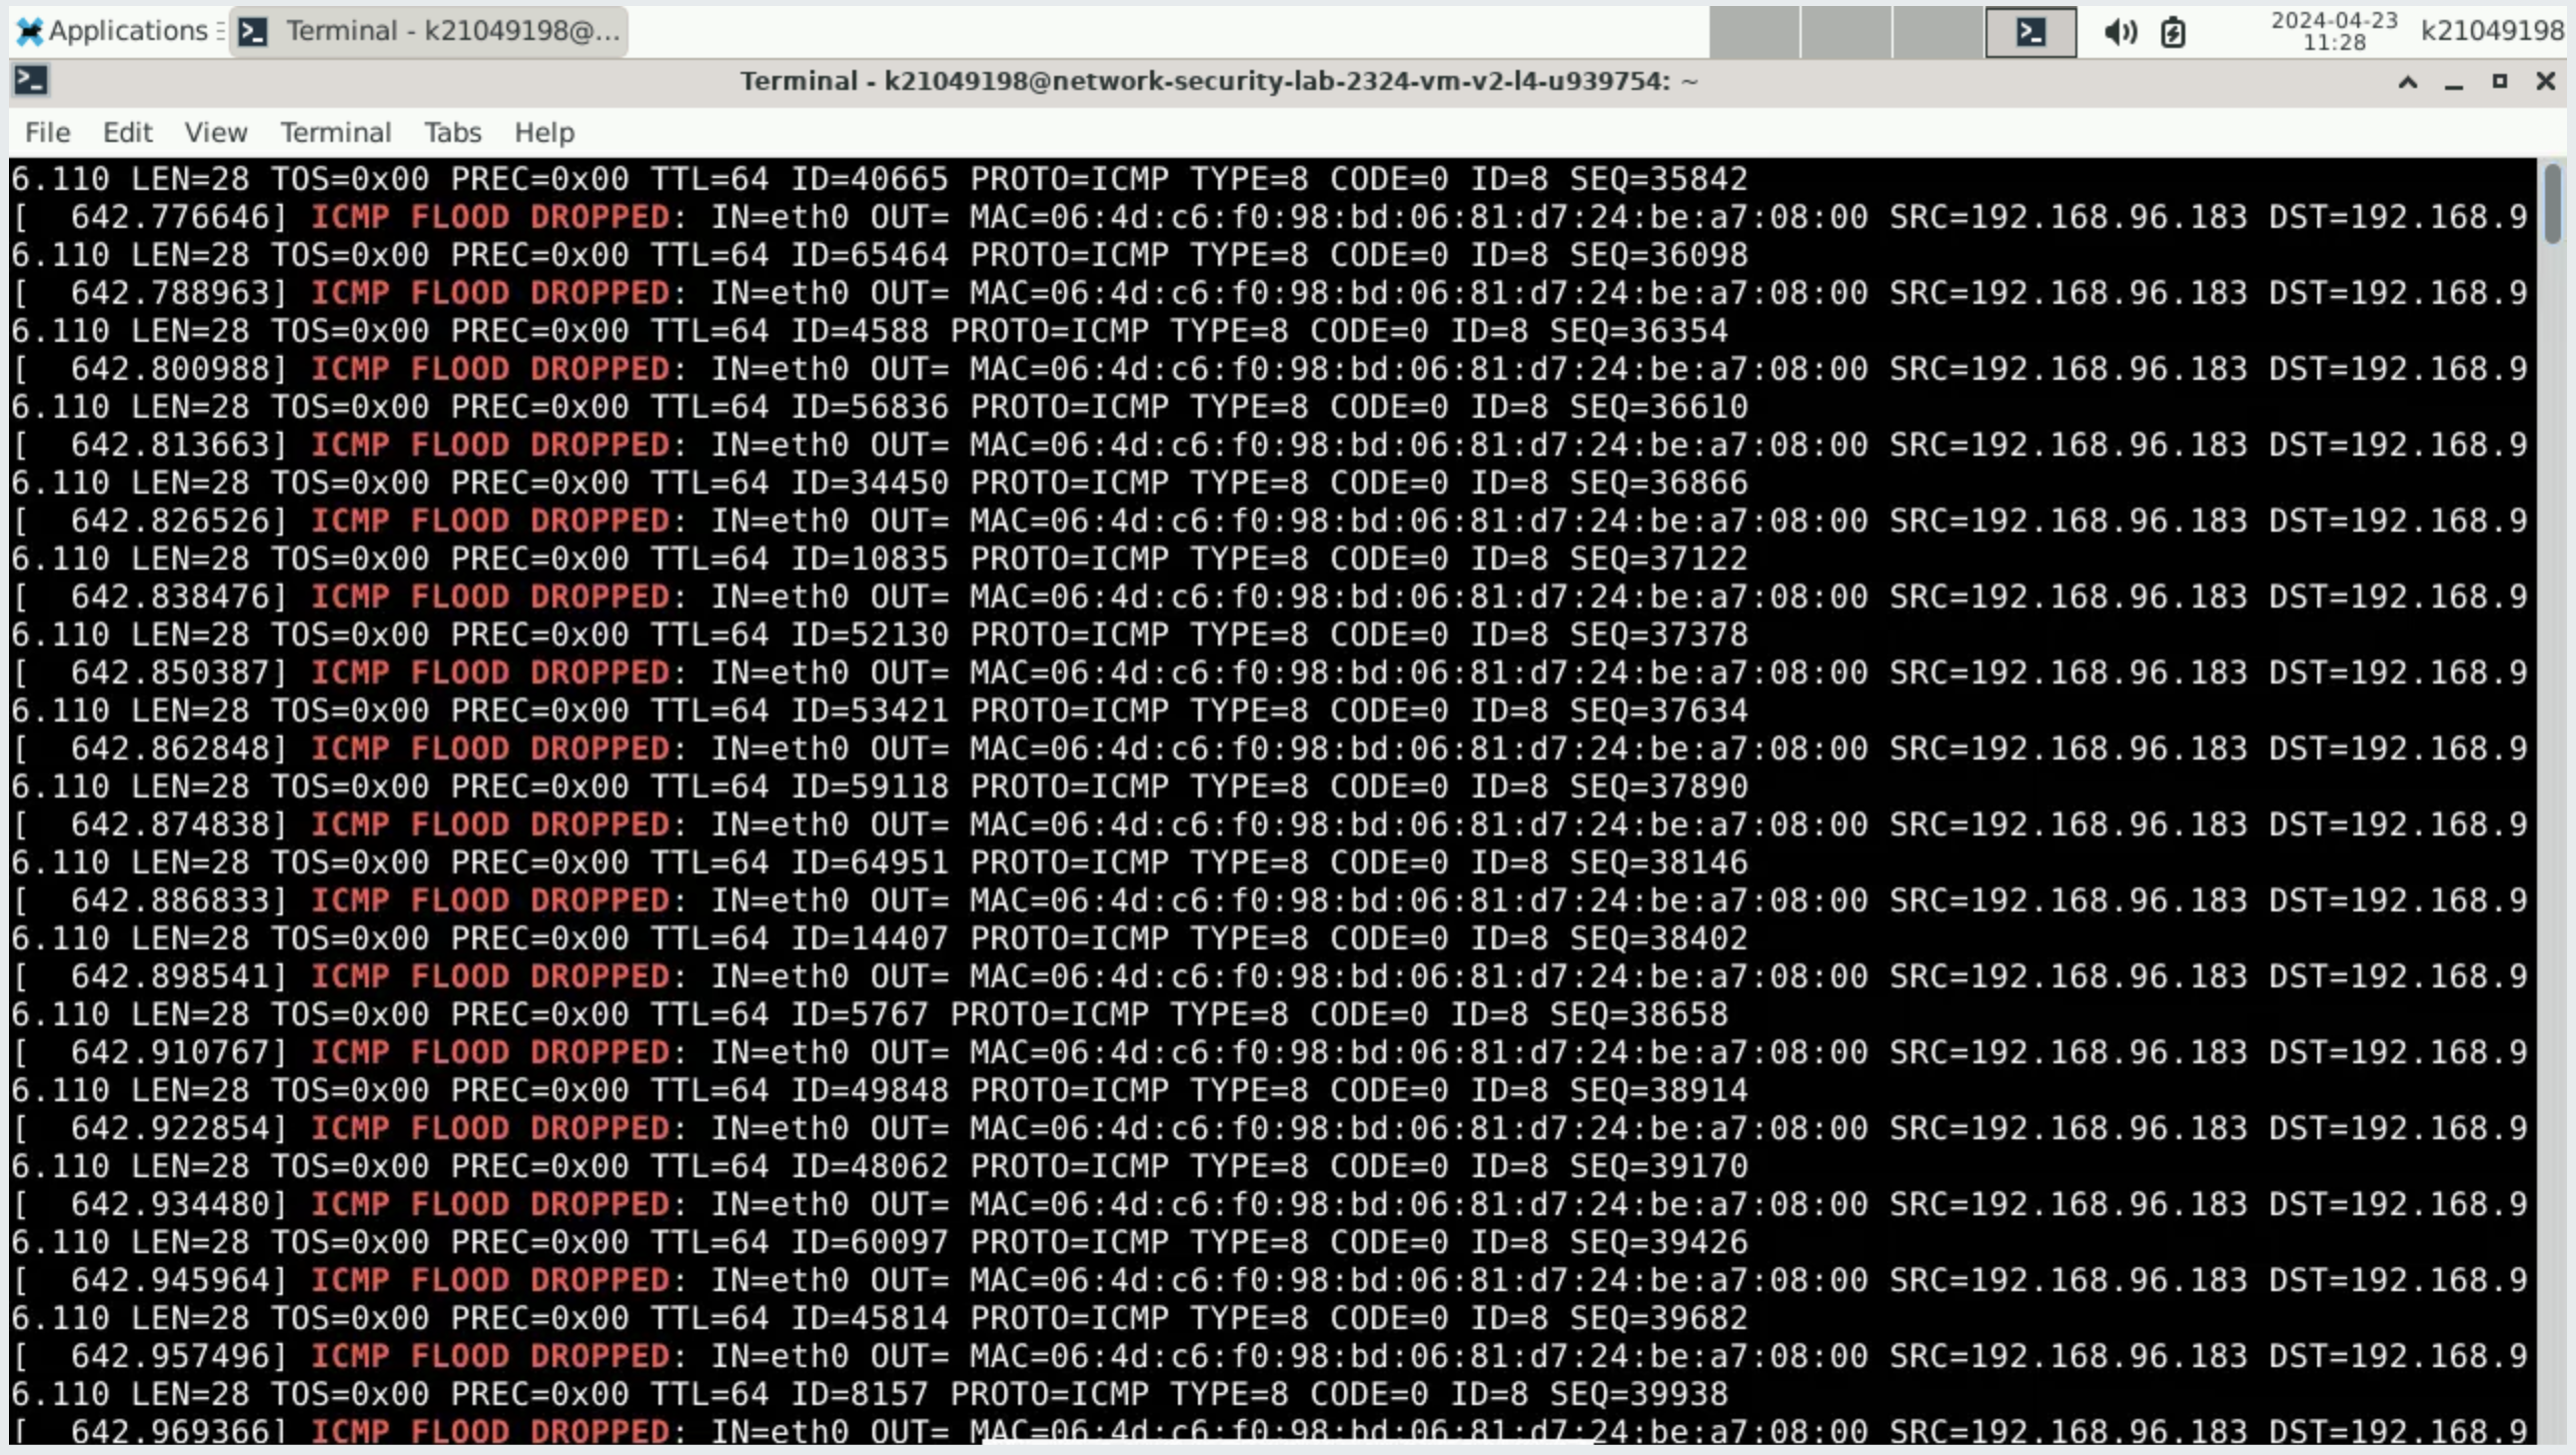
\includegraphics[width=0.8\textwidth]{img/level4/level4-dropped-packets-ICMPFlood.png}
\caption{Dropped Packets (ICMP Flood)}\label{fig:ICMPFloodDroppedPackets}
\end{figure}

\section{Performance Metrics}
To evaluate the firewall's impact on network performance during the attacks, we measured key performance metrics using \texttt{iperf}.

Figure~\ref{fig:TCPSYNFloodPerformanceMetrics} presents the performance metrics for the TCP SYN Flood attack scenario. Despite the attack, the firewall managed to maintain a relatively stable throughput, indicating its effectiveness in mitigating the impact of the attack on the network performance.

\begin{figure}[H]
\centering
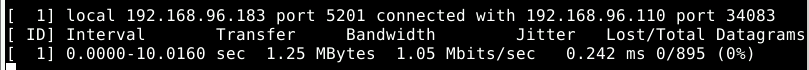
\includegraphics[width=0.8\textwidth]{img/level4/level4-performance-metrics-TCPSYNFlood.png}
\caption{Performance Metrics (TCP SYN Flood)}\label{fig:TCPSYNFloodPerformanceMetrics}
\end{figure}

Similarly, Figure~\ref{fig:ICMPFloodPerformanceMetrics} shows the performance metrics for the ICMP Flood attack scenario. The firewall successfully maintained the network performance, ensuring that the attack did not significantly affect legitimate traffic.

\begin{figure}[H]
\centering
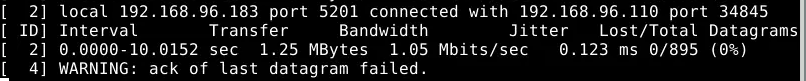
\includegraphics[width=0.8\textwidth]{img/level4/level4-performance-metrics-ICMPFlood.png}
\caption{Performance Metrics (ICMP Flood)}\label{fig:ICMPFloodPerformanceMetrics}
\end{figure}